\section{Quantum Modular Addition}
\label{sec:csa-mod-add}

To perform addition of two numbers $a$ and $b$ modulo $m$,
we consider the variant problem of modular addition of three numbers to
two numbers:
%
%\begin{quote}
Given three $n$-bit input numbers $a$, $b$, and $c$, and an $n$-bit modulus $m$,
compute
%\begin{equation}
$(u+v) = (a+b+c)[m]$,
%\end{equation}
where $(u+v)$ is a CSE number.

In this section, we provide an alternate, pedagogical explanation of
Gossett's modular reduction \cite{Gossett1998}. Later, we contribute a mapping of this adder
to a 2D architecture,
using unbounded fanout to maintain constant depth for adding back
modular residues. This last step is absent in Gossett's original approach.

To start, we will demonstrate the basic method of modular addition and reduction
on an $n$-bit conventional number. In general, adding two $n$-bit conventional
numbers will produce an overflow bit of significance $2^n$, which we can truncate as long as
we add back its modular residue $2^n \bmod m$. How can we guarantee that we won't
generate another overflow bit by adding back the modular residue? It turns out
we can accomplish this by allowing
a slightly larger input and output number ($n+1$ bits in this case), truncating
multiple overflow bits, and adding back their $n$-bit modular residues.

For two $(n+1)$-bit conventional numbers $x$ and $y$,
we truncate the three high-order bits of their sum $z_{n-1,n+3}$
and
add back their modular residue $x_{(n-1,n)}[m]$:
%
\begin{eqnarray}
x + y \bmod m &=& z_{(0,n+1)}[m] \nonumber \\
&=& z_{(0,n-2)} + z_{(n-1,n+1)}[m].
\end{eqnarray}
%
Since both the truncated number $z_{(0,n-2)}$ and the modular residue
are $n$-bit numbers, their sum is an $(n+1)$-bit number as desired, equivalent
to $x[m]$.

Now we must do the same modular reduction on a CSE number $(u+v)$,
which in this case represents an $(n+2)$-bit conventional number and has
$2n+3$ bits.
%This is the special case mentioned in the
%previous
%section \label{star:csa-special}, where $x$ is the result of a single
%CSA layer, not repeated CSA layers alternating with truncation.
%
%Assume for now that this modular reduction works;
%in the next section we walk through an illustrated concrete example.
%We present a more formal argument in Section \ref{subsec:mod-reduce-1}.
%
First, we truncate the three high-order bits ($v_{n}, u_{n-1}, v_{n-1}$)
of $(u+v)$, yielding an $n$-bit
conventional number with a CSE representation of $2n$ bits:
$\{u_0, u_1, \ldots, u_{n-1}\} \cup \{v_1, v_2, \ldots, v_{n-1}\}$.
Then we add back the three modular residues
$(v_{(n+1)}[m], u_{(n)}[m], v_{(n)}[m])$, and we are guaranteed not to
generate additional overflow bits (of significance $2^{n}$ or higher). This equivalence
is shown in Equation \ref{eqn:mod-reduce}.
\begin{eqnarray}
(u+v)[m] &=& \left(u_{(0,n+1)} + v_{(1,n+2)}\right)[m] \nonumber \\
 &=& u_{(0,n)} +
     v_{(1,n)} + \nonumber \\
 & & u_{(n+1)}[m] +
     v_{(n+1)}[m] + v_{(n+2)}[m]
\label{eqn:mod-reduce}
\end{eqnarray}

\begin{lemma}[Modular Reduction in Constant Depth]
The modular addition of three $n$-bit numbers to two $n$-bit numbers can be
accomplished
in constant depth with $O(n)$ width in \textsc{2D CCNTC}.
\end{lemma}

\begin{proof}
Our goal is to show how to perform modular addition while keeping our numbers
of a fixed size by treating overflow bits correctly.
We map the proof of \cite{Gossett1998} to \textsc{2D CCNTC} and show that
we meet our required depth and width.
First, we enlarge our registers to allow the addition of $(n+2)$-bit numbers,
while keeping our modulus of size $n$ bits.
(In Gossett's original approach, he takes the equivalent step of restricting
the modulus to be of size $(n-2)$ bits.) We accomplish the modular addition
by first performing a layer of non-modular addition, truncating the three high-order
overflow bits, and then adding back modular residues controlled on these
bits in three successive layers, where we are guaranteed that no additional
overflow bits are generated in each layer.
This is illustrated for a $3$-bit modulus and $5$-bit registers
in Figure \ref{fig:csa-proof}.

\begin{center}
\begin{figure*}[h!tb]
\begin{displaymath}
\renewcommand\arraystretch{1.5}
\begin{array}{ccccccll}
        & a_4 & a_3 & a_2 & a_1 & a_0 & 5\text{-bit input number } a &\\
        & b_4 & b_3 & b_2 & b_1 & b_0 & 5\text{-bit input number } b & \\
        & c_4 & c_3 & c_2 & c_1 & c_0 & 5\text{-bit input number } c & \text{[Layer 1]}\\
\hline
        & u_4 & u_3 & u_2 & u_1 & u_0 & \text{truncate } u_{4} & \\
    v_5 & v_4 & v_3 & v_2 & v_1 &     & \text{truncate } v_{4},v_{5} & \\
        &     &     & c^{v_4}_2 & c^{v_4}_1 & c^{v_4}_0 & \text{add back } 2^4 \bmod m \text{ controlled on } v_4 & \text{[Layer 2]}\\
\hline
        &      & u'_3 & u'_2 & u'_1 & u'_0 & & \\
        & v'_4 & v'_3 & v'_2 & v'_1 &      & & \\
        &      &    & c^{u_4}_2 & c^{u_4}_1 & c^{u_4}_0  & \text{add back } 2^4 \bmod m \text{ controlled on } u_4 & \text{[Layer 3]}\\
\hline
        & u''_4 & u''_3 & u''_2 & u''_1 & u''_0 & \text{the bit } u''_4 \text{ is the same as } v'_4 & \\
        & v''_4 & v''_3 & v''_2 & v''_1 &       &  & \\
        &       &    & c^{v_5}_2 & c^{v_5}_1 & c^{v_5}_0 & \text{add back } 2^5 \bmod m \text{ controlled on } v_5 & \text{[Layer 4]}\\
\hline
        & u'''_4 & u'''_3 & u'''_2 & u'''_1 & u'''_0 & \text{ Final CSE output with } 5 \text{ bits} &\\
        & v'''_4 & v'''_3 & v'''_2 & v'''_1 &        & \text{ Final CSE output with } 5 \text{ bits} & \\
\end{array}
%\begin{array}{cccccccr}
%        & a_{n+1} & a_{n} & a_{n-1} & \ldots & a_1 & a_0 & \text{input number } a\\
%        & b_{n+1} & b_{n} & b_{n-1} & \ldots & b_1 & b_0 & \text{input number } b\\
%        & c_{n+1} & c_{n} & c_{n-1} & \ldots & c_1 & c_0 & \text{input number } c\\
%\hline
%        & u_{n+1} & u_{n} & u_{n-1} & \ldots & u_1 & u_0 & \text{truncate } u_{n+1} \\
%v_{n+2} & v_{n+1} & v_{n} & v_{n-1} & \ldots & v_1 & 0   & \text{truncate } v_{n+1},v_{n+2} \\
%        &         &       & x_{n-1} & \ldots & x_1 & x_0 \\
%\hline
%        &         & u'_{n} & u'_{n-1} & \ldots & u'_1 & u'_0 & \\
%        & v'_{n+1} & v'_{n} & v'_{n-1} & \ldots & v'_1 & 0 &  \\
%        &         &       & x_{n-1} & \ldots & x_1 & x_0 \\
%\hline
%        & u''_{n+1} & u''_{n} & u''_{n-1} & \ldots & u''_1 & u''_0 & \\
%        & v''_{n+1} & v''_{n} & v''_{n-1} & \ldots & v''_1 & 0 &  \\
%        &         &       & y_{n-1} & \ldots & y_1 & y_0 \\
%\hline
%        & u'''_{n+1} & u'''_{n} & u'''_{n-1} & \ldots & u'''_1 & u'''_0 & \\
%        & v'''_{n+1} & v'''_{n} & v'''_{n-1} & \ldots & v'''_1 & 0 &  \\
%\hline
%\end{array}
\end{displaymath}
\caption{A schematic proof of Gossett's constant-depth modular reduction for $n=3$.}
\label{fig:csa-proof}
\end{figure*}
\end{center}

We use the following notation.
The non-modular sum of the first layer is $u$ and $v$.
The CSE output of the first modular reduction layer
is $u'$ and $v'$, and the modular residue is
written as $c^{v_{n+1}}$ to mean the precomputed value $2^{n+1} \bmod m$
controlled on $v_{n+1}$.
The CSE output of the second modular reduction layer
is $u''$ and $v''$, and the modular residue is written as
$c^{u_{n+1}}$ to mean the precomputed value $2^{n+1} \bmod m$
controlled on $u_{n+1}$.
The CSE output of the third and final modular reduction layer
is $u'''$ and $v'''$, and the modular residue is written as
$c^{v_{n+2}}$ to mean the precomputed value $2^{n+2} \bmod m$
controlled on $v_{n+2}$.

We show that no layer generates an overflow $(n+2)$-bit, namely in the
$v$ component of any CSE output. (The $u$ component will never exceed the
size of the input numbers.) First, we know that no $v'_{n+2}$ bit
is generated after the first modular reduction layer, because we have
truncated away all $(n+1)$-bits. Second, we know that no $v''_{n+2}$ bit is
generated because we only have one $(n+1)$-bit to add, $v'_{n+1}$.
Finally, we need to show that $v'''_{n+2} = 0$ in the third modular reduction
layer. 

Since $u'_{(n)} + v'_{(n+1)} =
u_{(n)} + v_{(n)} \le 2^{n+1}$, the bits $u'_n$ and $v'_{n+1}$ cannot both be $1$.
But $u''_{n+1} = v'_{n+1}$ and $v''_{n+1} = u'_n\land v'_n$, so $u''_{n+1}$ and
$v''_{n+1}$ cannot both be $1$, and hence $v'''_{n+2} = 0$.
%This bit is the majority of
%$u''_{n+1}$, $v''_{n+1}$, and $c^{v_{n+2}}_{n+1} = 0$. This means we only have
%to guarantee that at most one of $u''_{n+1}$ and $v''_{n+1}$ has value 1.
%This is equivalent to requiring that
%$u''_{(n,n+1)} + v''_{(n+1)} \le 3\cdot 2^{n}$, that is, the sum of these
%three bits has value at most $3$. Bit $u''_{n+1}$ is copied directly from
%$v'_{n+1}$ by the rules of CSA, which requires the following condition for
%the second modular reduction layer:
%$u'_{(n)} + v'_{(n,n+1)} \le 3\cdot 2^n$. This is true because
%$u'_{(n)} + v'_{(n+1)} = u_{(n)} + v_{(n)} \le 2$ and $v'_{(n)} \le 1$.
Everywhere
we use the fact that the modular residues are restricted to $n$ bits.
Therefore, the modular sum is computed as the sum of two $(n+2)$-bit numbers
with no overflows in constant-depth.
\end{proof}

As a side note, we can perform modular reduction in one layer instead of
three by decoding the three overflow bits into one of seven different
modular residues. This can also be done in constant depth, and in this case
we only need to enlarge all our registers to $(n+1)$ bits instead of $(n+2)$
as in the proof above. We omit the proof for brevity.

In the following two subsections, we give a concrete example to illustrate
the modular addition circuit as well as a numerical upper bound for the
general circuit resources.

%%%%%%%%%%%%%%%%%%%%%%%%%%%%%%%%%%%%%%%%%%%%%%%%%%%%%%%%%%%%%%%%%%%%%%%%%%%%%%%
\subsection{A Concrete Example of Modular Addition}
\label{subsec:concrete}

\begin{center}
\begin{figure*}[h!bt]
\centerline{
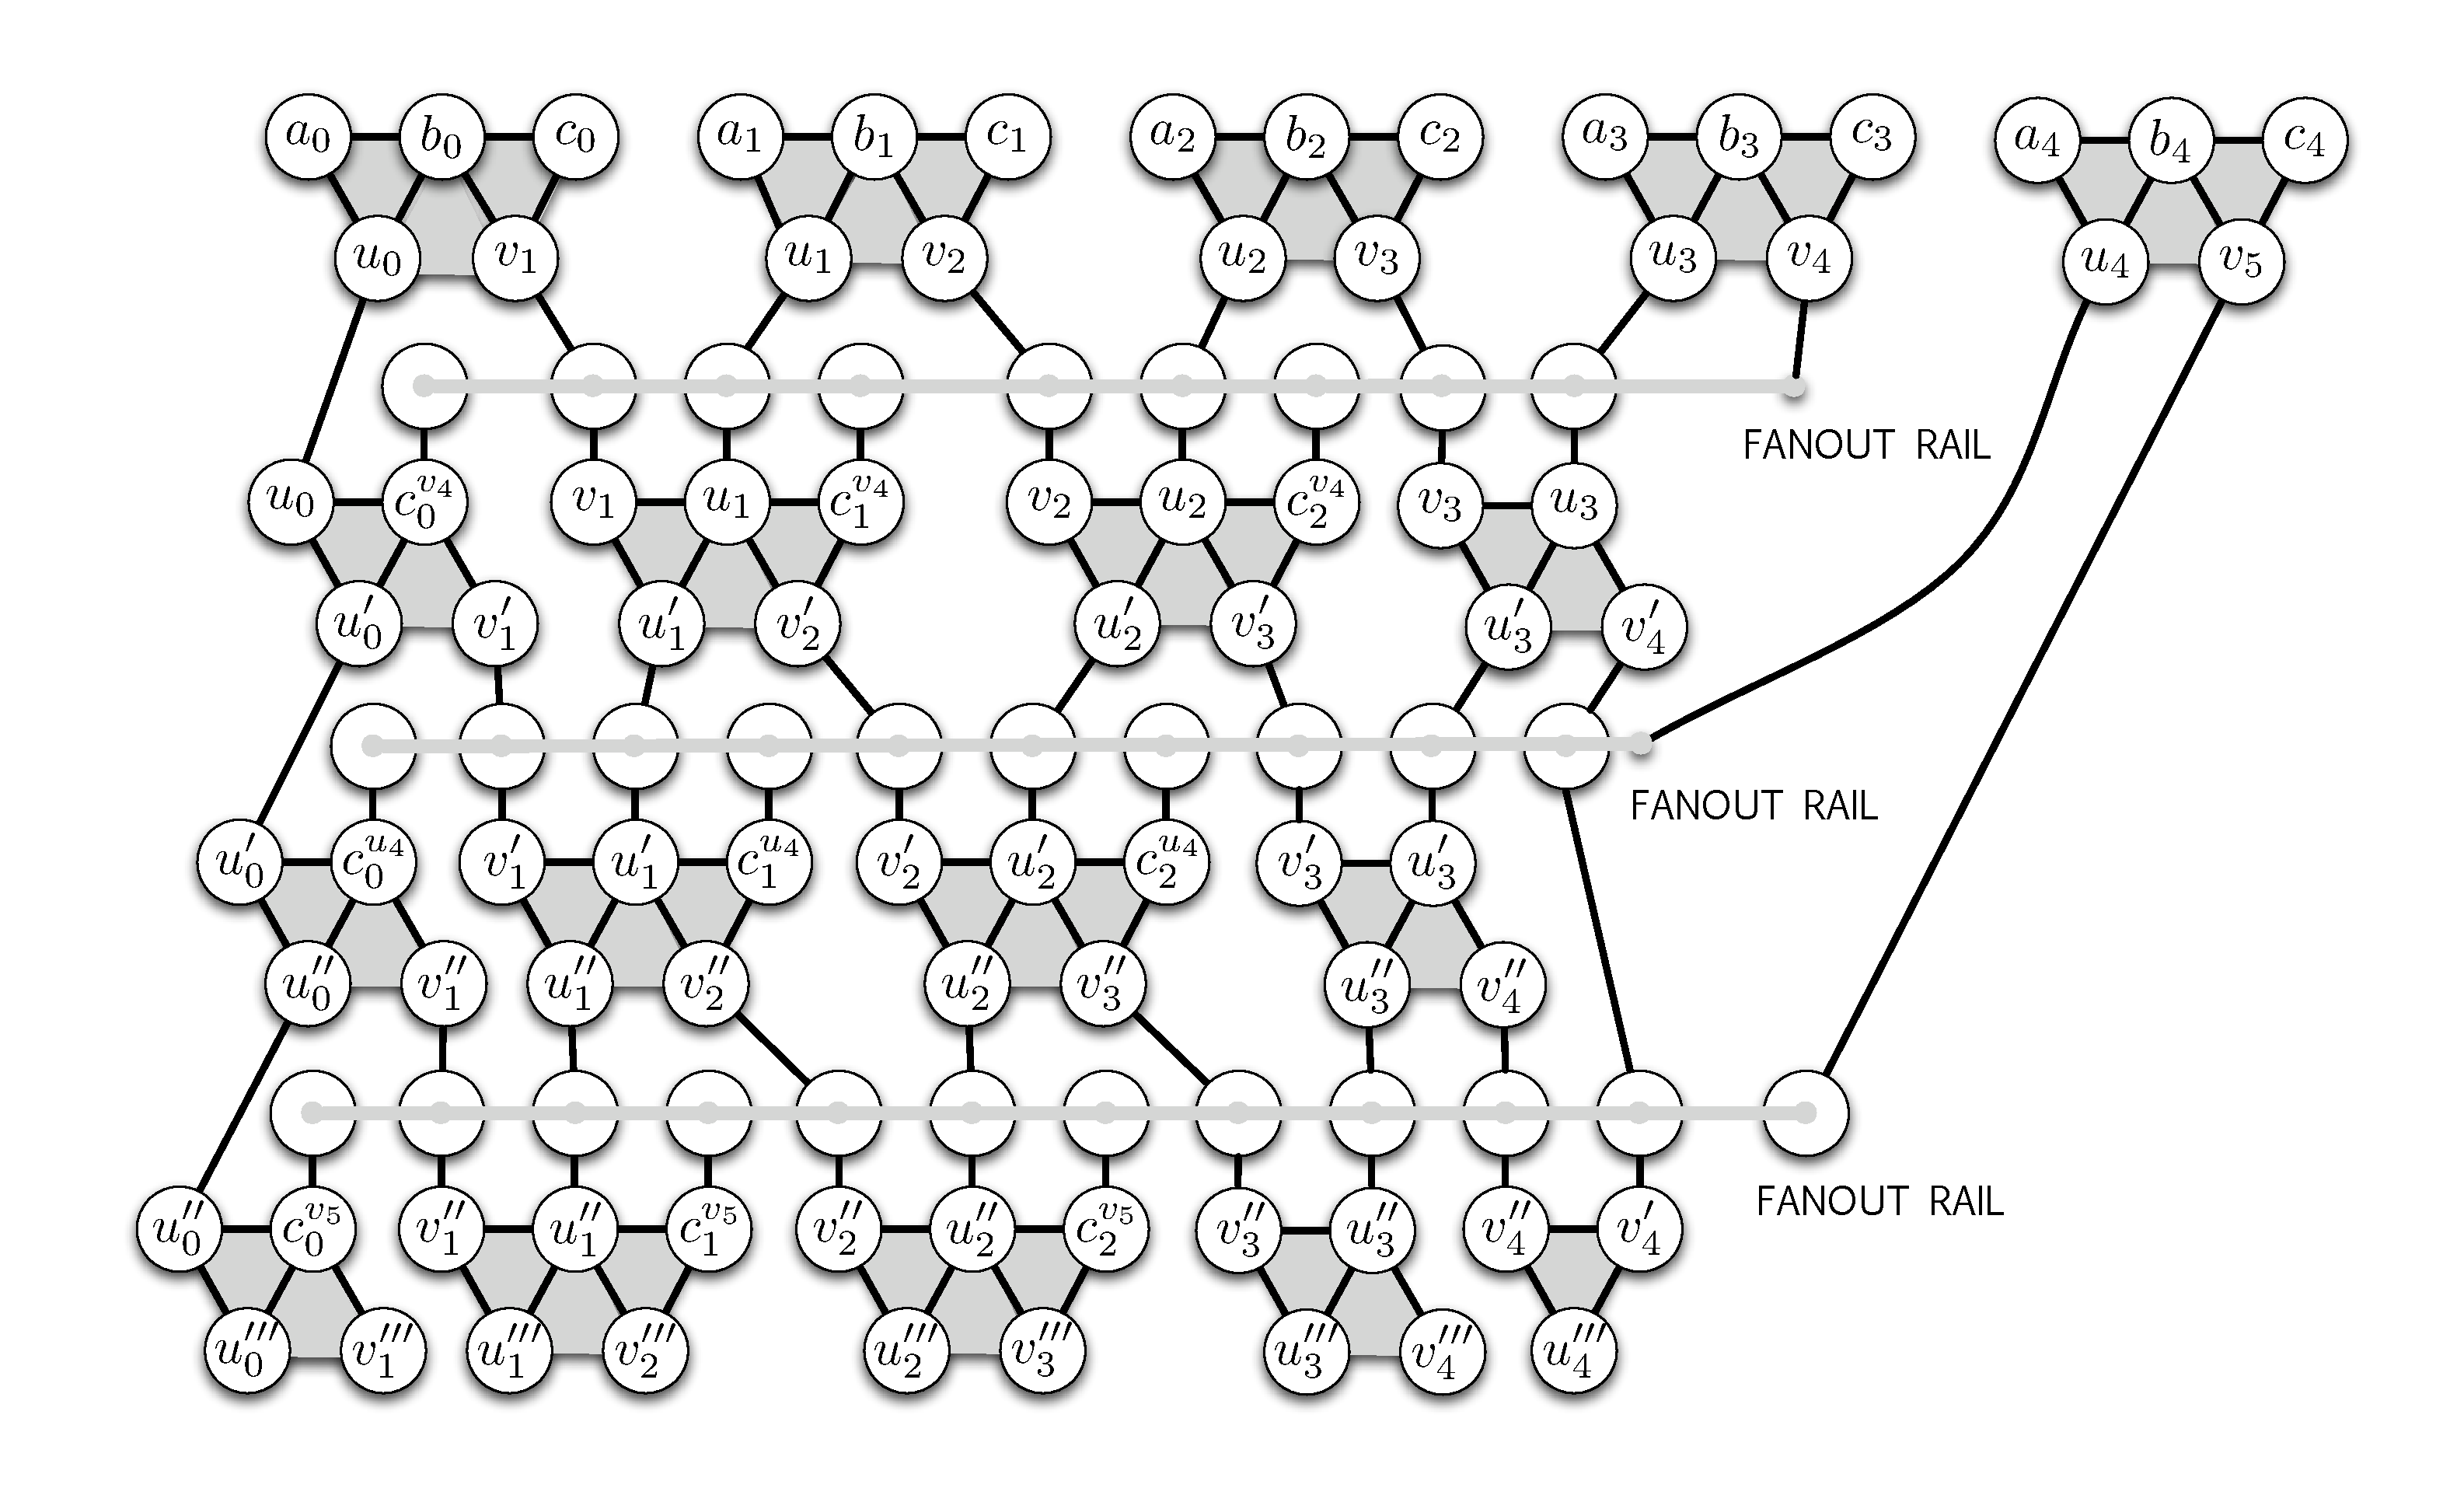
\includegraphics[width=6.5in]{factor-polylog/figures/mod-add-fixed.pdf}
}
\caption{Addition and three rounds of modular reduction for a 3-bit
modulus.}
\label{fig:csa-add-4}
\end{figure*}
\end{center}

A \textsc{2D CCNTC} circuit for modular addition of $5$-bit numbers using
four layers of parallel CSA's is shown graphically in Figure \ref{fig:csa-add-4}
which corresponds directly to the schematic proof in Figure \ref{fig:csa-proof}.
Note that in Figure \ref{fig:csa-add-4}, the least significant qubits are
on the left, and in Figure \ref{fig:csa-proof}, the least significant qubits are
on the right.
Figure \ref{fig:csa-add-4} also represents the approximate
physical layout of the qubits as they would look if this
circuit were to be fabricated.
Here, we convert the sum of three
$5$-bit integers into the modular sum of two $5$-bit integers, with a
$3$-bit modulus $m$.
In the first layer,
we perform 4 CSA's in parallel on the input numbers ($a,b,c$) and produce the
output numbers ($u, v$).

As described above, we truncate
the three high-order bits during the initial CSA round
(bits $u_4, v_4, v_5$) to retain a $4$-bit number.
Each of these bits serves as a control for adding its modular residue to
a running total. We can classically precompute $2^4[m]$ for the two
additions controlled on $u_4$ and $v_4$ and
$2^5[m]$ for the addition controlled on $v_5$.

In Layer 2,
we use a constant-depth fanout rail (see Figure \ref{fig:cdf}) to
distribute the control bit $v_4$ to its modular residue, which we denote as
%%\begin{equation}
$\ket{c^{v_4}} \equiv \ket{2^4[m]\cdot v_4}$.
%%\end{equation}
%This fanout requires constant depth;
The register $c^{v_4}$ has $n$ bits, which we add to the CSE results of layer 1.
The results $u_i$ and $v_{i+1}$ are teleported into layer 3. The exception is
$v'_4$ which is teleported into layer 4, since there are no other $4$-bits
to which it can be added. Wherever there are only
two bits of the same significance, we use the 2-2 adder from
Section \ref{sec:csa}.

Layer 3
%%, shown in Figure \ref{fig:csa-add-3},
operates similarly to layer 2, except that the modular residue is controlled on
$u_4$:
%%\begin{equation}
$\ket{c^{u_4}} \equiv \ket{2^4[m] \cdot u_4}$.
%%\end{equation}
%This fanout again requires constant depth;
The register $c^{u_4}$ has $3$ bits, which we
add to the CSE results of layer 2, where $u'_i$ and $v'_{i+1}$ are teleported
forward into layer 4.

Layer 4
%%, shown in Figure \ref{fig:csa-add-4},
is similar to layers 2 and 3, with the modular residue controlled on $v_5$:
%%\begin{equation}
$\ket{c^{v_5}} \equiv \ket{2^5[m] \cdot v_5}$.
%%\end{equation}
%This fanout is constant depth;
The register $c^{v_5}$ has $3$ bits, which we
add to the CSE results of layer 3.
There is no overflow bit $v'''_5$, and no carry bit from $v''_4$ and $v'_4$
as argued in the proof of Lemma 1.
The final modular sum $(a+b+c)[m]$ is $u'''+v'''$.

The general circuit for adding three $n$-qubit quantum integers to
two $n$-qubit quantum integers is called a \emph{CSA tile}. Each CSA tile in our architecture 
corresponds to its own module, and it will be represented by the symbol in 
Figure \ref{fig:csa-tile-symbol} for the rest of this paper. We call this
an $n$-bit modular adder, even though it accepts $(n+2)$-bit inputs, because
the size of the modulus is still $n$ bits.

\begin{center}
\begin{figure*}[h!bt]
\centerline{
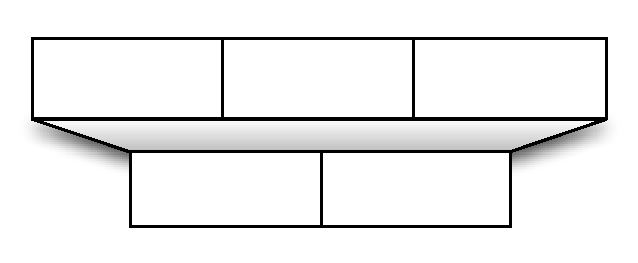
\includegraphics[width=1.5in]{factor-polylog/figures/csa-tile-symbol.pdf}
}
\caption{Symbol for an $n$-bit 3-to-2 modular adder, also called a CSA tile.}
\label{fig:csa-tile-symbol}
\end{figure*}
\end{center}


\subsection{Quantum Circuit Resources for Modular Addition}

We now calculate numerical upper bounds for the circuit resources of
the $n$-bit $3$-to-$2$ modular adder described in the previous section.
There are four layers of non-modular $n'$-bit $3$-to-$2$ adders, each of which
consists of $n'$ parallel single-bit adders whose
resources are detailed in Table \ref{tab:csa-tile-resources}. For factoring
an $n$-bit modulus, we have $n'=n+2$ in the first and fourth layers
and $n'=n+1$ in the second and third layers.

After each of the first three layers, we must move the output qubits
across the fanout rail to be the inputs of the next layer. We use
two swap gates, which have a depth and size of $6$ CNOTs each, since
the depth of teleportation is only more efficient for moving more than
two qubits. The control bit for each modular residue needs to be
teleported $0$, $4$, and $7$ qubits respectively according to the
diagram in Figure \ref{fig:csa-add-4}, before being fanned out $n$
times along the fanout rails, where the fanned out copies will end up
in the correct position to be added as inputs.

%The detailed resources for a Toffoli gate and the single-bit adder that uses
%them are given in Table \ref{tab:csa-tile-resources}.

The resources for the $n$-bit $3$-to-$2$ modular adder depicted in Figure
\ref{fig:csa-add-4} are given below.
The formulae reflect the resources needed for both computing the output
in the forward direction (including creating an entangled fanned-out state
controlled on overflow qubits)
and also uncomputing ancillae in the backward
direction (including disentangling previous fanned-out copies).

The circuit depth is $O(1)$:

\begin{equation}
374\text{.}
\end{equation}

The circuit size is $O(n)$:

\begin{equation}
551n + 757\text{.}
\end{equation}

The circuit width is $O(n)$:

\begin{equation}
33n + 47\text{.}
\end{equation}